A $\beta$-strand is a polypeptide chain that is almost fully extended, 
with the sidechains of neighbouring residues directed in opposite orientations (Fig. \ref{fig:sheet}). 
Folding the chain back and forth brings $\beta$-strands next to each other, 
which allows them to undergo hydrogen bonding and form a $\beta$-sheet.
Adjacent residues along the strand point in opposite directions and the distance between them is 3.5 Å. 
Neighbouring strands either run in the same or opposite directions. 
This forms a antiparallel, parallel, or mixed $\beta$-sheet
In antiparallel arrangement (middle and bottom strand),
the NH group and CO group of an amino acid are hydrogen bonded with a partner amino acid in the neighbouring strand.
The parallel arrangement is more complicated.
Each amino acid of one strand forms hydrogen bonds with two amino acids of the adjacent strand. 
Finally, in the mixed sheet parallel and antiparallel neighbouring strands are mixed in one sheet
(\cite{berg2015}).

~\begin{figure}[h!]
	\centering
	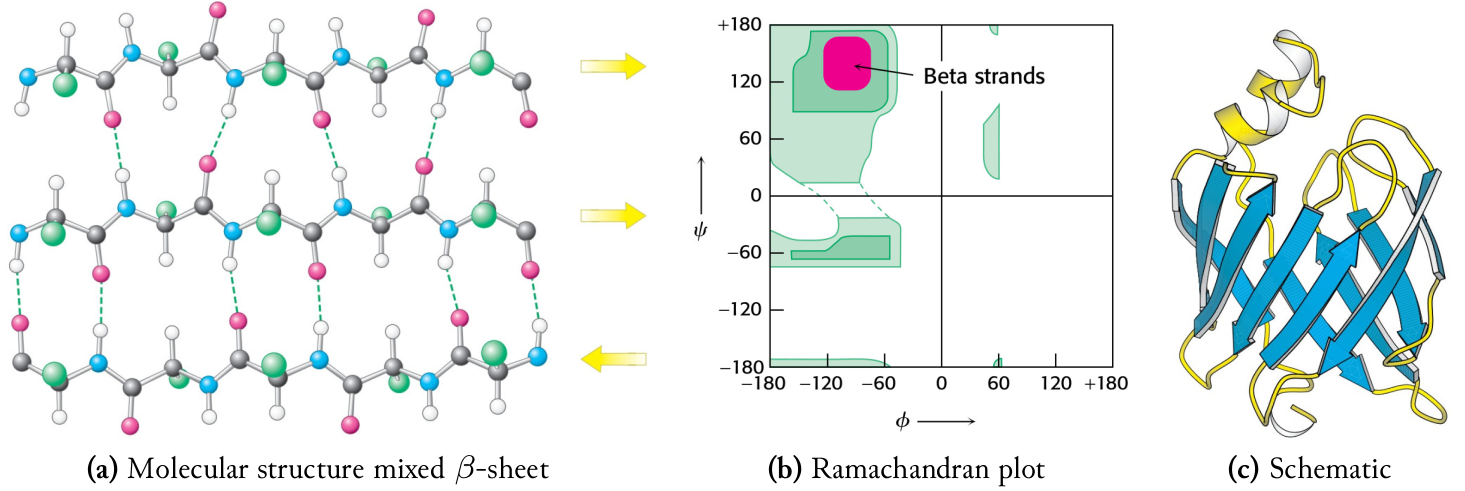
\includegraphics[width=\linewidth]{./literature_review/proteins/secundary_structure/sheet/img/sheet.png}
	\caption{
		\textbf{$\beta$-sheet secondary structure. a.}
	Molecular structure of a mixed $\beta$-sheet. 
	Adjacent residues along the strand point in opposite directions and the distance between them is 3.5 Angstron. 
	In antiparallel arrangement (middle and bottom strand),
	the NH group and CO group of an amino acid are hydrogen bonded with a partner amino acid in the neighbouring strand.
	The parallel arrangement is more complicated (top strand and middle strand). 
	Each amino acid of one strand forms hydrogen bonds with two amino acids of the adjacent strand. 
	Green:R-group, 
	Black:Carbon, 
	Purple:Oxygen, 
	Blue:Nitrogen,
	White:Hydrogen, 
		\textbf{b.}
	Situation of $\psi$ and $\phi$ angles of the $\beta$-strand on the Ramachandran plot.
		\textbf{c.}
	Schematic representation of a protein rich in $\beta$-sheets.
	}
	\label{fig:sheet}
~\end{figure}
